%!TEX root = ../DigSig2.tex
\section{Signal Processing Applications\buch{Chapter 8}}
\subsection{Digital Waveform Generators\buchSeite{316}}

The goal is to design a filter $H(\z)$ with a desired impulse response $h(n)$.

\begin{center}
	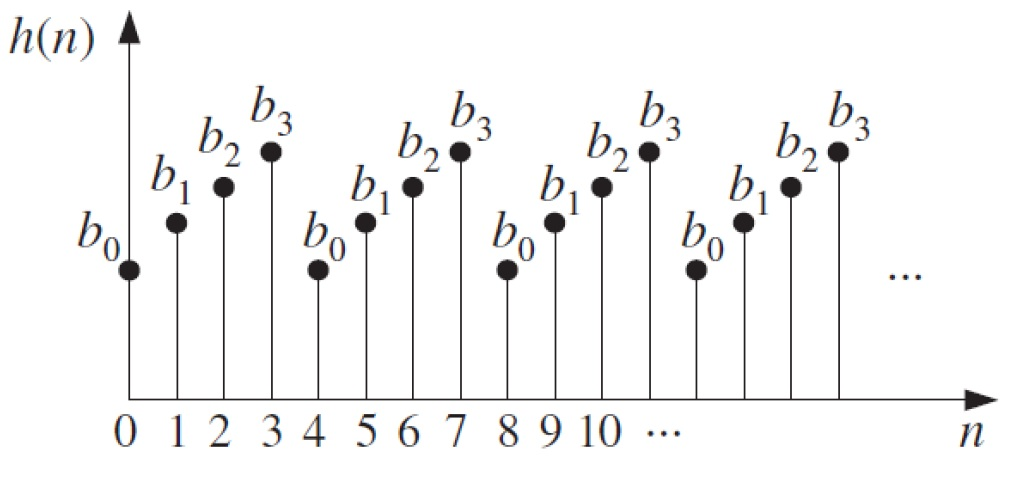
\includegraphics[width=6cm]{images/SignProcApp_DigWaveFormGenerator.jpg}
\end{center}
This waveform can be sample-by-sample computed as the impulse response of the filter $H(\z)$ or it can be pre-computed and stored in memory (wavetable).
If the waveform is periodic (often) then the fundamental frequency can be controlled by the speed the wavetable is read out.

\subsubsection{Sinusodial Generators\buchSeite{316-320}}
A causal sinusoidal is implemented by
\begin{align*}
	h(n) &= R^n \sin(\omega_0 n)u(n) \\
	H(\z) &= \frac{R \sin \omega_0 \z^{-1}}{1-2R\cos \omega_0 \z^{-1} + R^2 \z^{-2}}
\end{align*}
with $\omega_0 = 2 \pi f_0 / f_s$ being the digital frequency. \\

For $R=1$, $h(n)$ is a pure sine, for $0<R<1$, $h(n)$ is a geometrically declining sinusoidal wave. \\

A cosinusoidal signal is generated similarly with
\begin{align*}
	h(n) &= R^n \cos(\omega_0 n)u(n) \\
	H(\z) &= \frac{1 - R \cos \omega_0 \z^{-1}}{1-2R\cos \omega_0 \z^{-1} + R^2 \z^{-2}}
\end{align*}

As the poles of the transfer functions are at conjugate complex locations, both generators can be combined to the \emph{coupled form}:

\begin{center}
	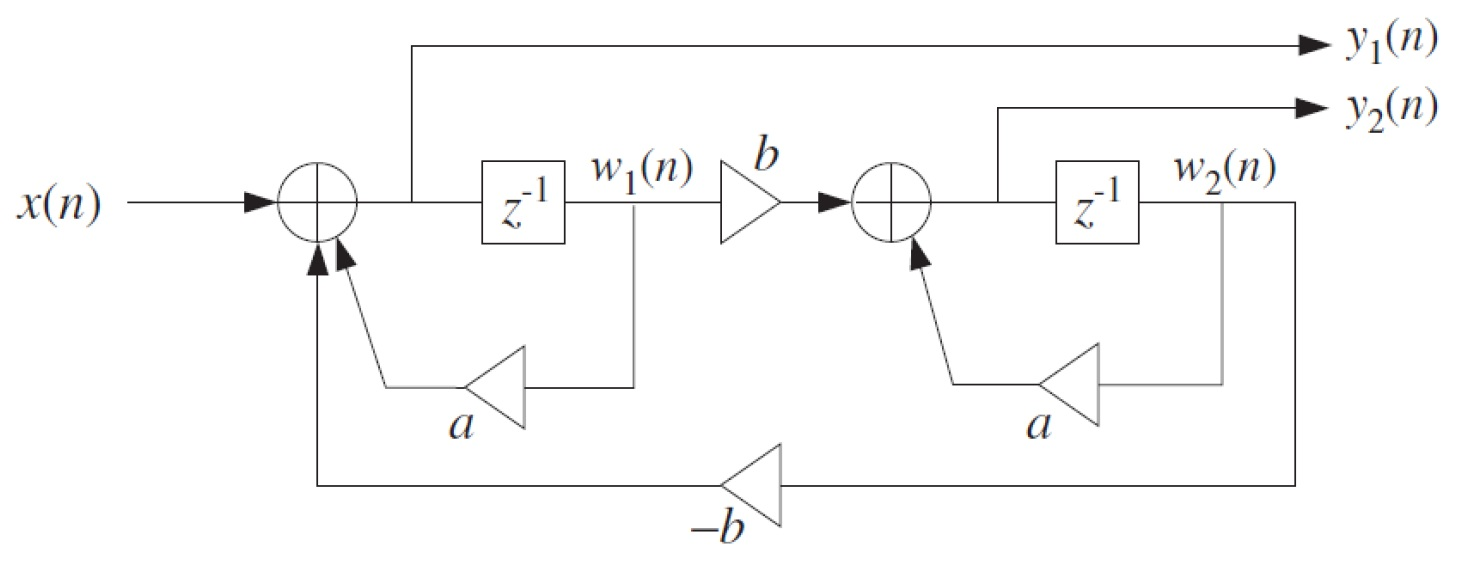
\includegraphics[width=\linewidth]{images/SignProcApp_SinCoupledForm.jpg}
\end{center}
with
\begin{equation*}
	a = R \cos \omega_0 \qquad b = R \sin \omega_0
\end{equation*}
or in the $z$-domain:
\begin{align*}
	H_1(\z) &= \frac{1 - a \z^{-1}}{1 - 2 a \z^{-1} + (a^2+b^2) \z^{-2}}  &\text{(cosine)} \\
	H_2(\z) &= \frac{b \z^{-1}}{1 - 2 a \z^{-1} + (a^2+b^2) \z^{-2}} &\text{(sine)}
\end{align*}

\subsubsection{Periodic Waveform Generators\buchSeite{321-329}}
A sampled version of a periodic signal is not necessarily periodic.
In order for $x(n)$ to be periodic in $n$ with a period of $D$ samples,
one whole period of the signal must fit within the $D$ samples.
Therefore at $n = D$ the signal must cycle by one whole period. \\

This requires that $x(D) = x(0)$, which requires
\begin{align*}
	\omega = \frac{2\pi}{D} && f = \frac{f_s}{D} && f_s = Df && T_D = DT
\end{align*}


Because of the periodicity, it is enough to specify the signal over one period only:
\begin{align*}
	h = [b_0, b_1, \ldots, b_{D-1}, \: b_0, b_1, \ldots, b_{D-1}, \: b_0, \ldots]
\end{align*}

With the corresponding z-transform:
\begin{align*}
	H(\z) = \frac{b_0 + b_1 \z^{-1} + b_2 \z^{-2} + \ldots + b_{D-1} \z^{-(D-1)}}{1 - \z^{-D}}
\end{align*}
or the impulse response
\begin{align*}
	h(0) &= b_0 \quad h(1) = b_1 \quad \ldots \quad h(D-1) = b_{D-1} \\
	h(n) &= h(n-D) \quad \text{for } n \geq D
\end{align*}

The canonical realization is the following:
\begin{center}
	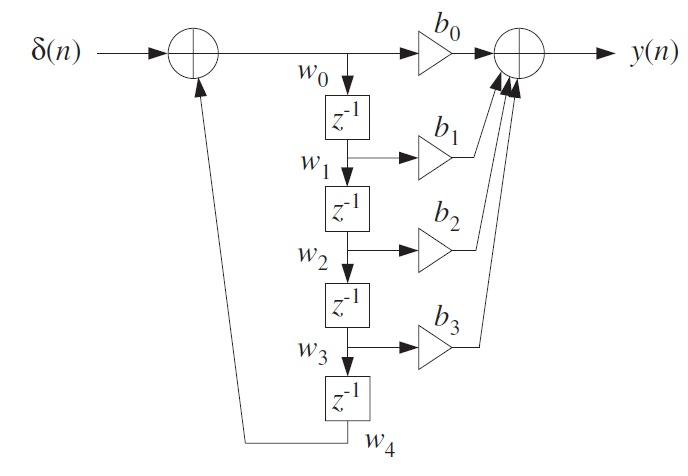
\includegraphics[width=\linewidth]{images/SignProcApp_PeriodicWaveFormGen.jpg}
\end{center}

The common delay line of the canonical form can be split up into two identical delay lines.
The first recursive filter creates a periodic impulse train as impulse response, which in turn creates a periodic waveform which consists of the finite impulse response of the FIR filter excited over and over again
\begin{center}
  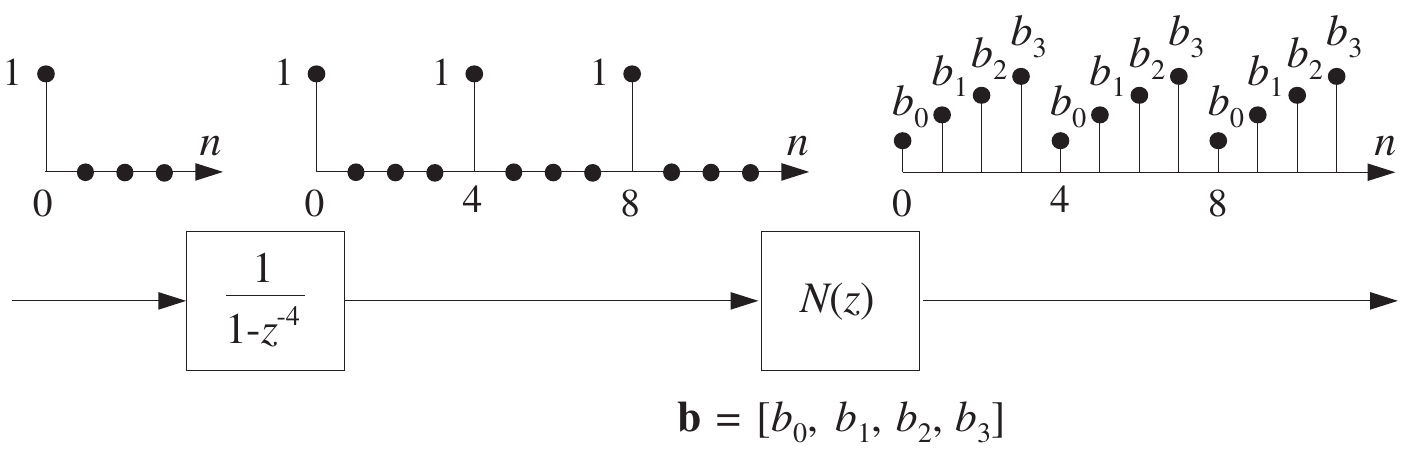
\includegraphics[width=\linewidth]{images/SignProcApp_ImpulseTrain.png}
\end{center}

These sequences are causal, therefore they have a comb-like spectra, with dominant peaks (poles) at the harmonics.
The spectrum can be obtained by setting $z=e^{jw}$ in the transfer function:
\begin{align*}
  1 - z^{-D} = ... &= 2je^{j\omega D/2}\text{sin}(\frac{\omega D}{2}) \\
  |H(\omega)| = \frac{|N(\omega)|}{|1-e^{-j\omega D}|} &= \frac{|N(\omega)|}{2|\text{sin}(\frac{\omega D}{2})|} \\
  \omega &= 2\pi f/f_s \\
  |H(f)| &= \frac{|N(f)|}{2|\underbrace{\text{sin}(\frac{\pi fD}{f_s})}_{=0}|} \\
  \Rightarrow \frac{\pi fD}{f_s} &= \pi m \\
  \Leftrightarrow f_m = m\frac{f_s}{D} = mf_1 &\quad f_1 \text{: fundamental frequency}
\end{align*}
\begin{center}
  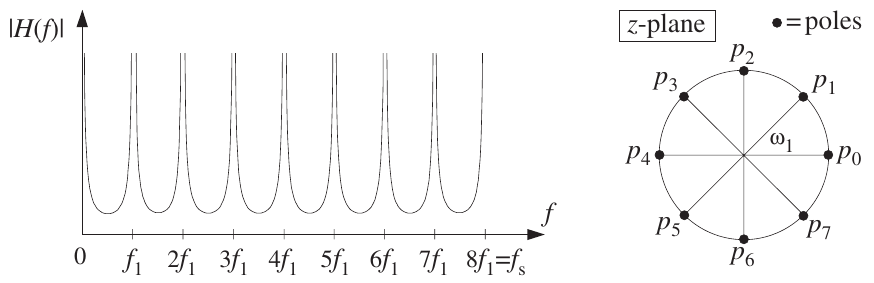
\includegraphics[width=\linewidth]{images/SignProcApp_Spectrum.png}
\end{center}


\subsubsection{Wavetable Generators\buchSeite{330-349}}
An alternative approach is to store the samples of a period in memory and
play this sample over and over again. This is called a wavetable $\mathbf{w}$. The readout is accomplished using a circular pointer $p$ and, if needed, an offset index $q$.

\begin{center}
	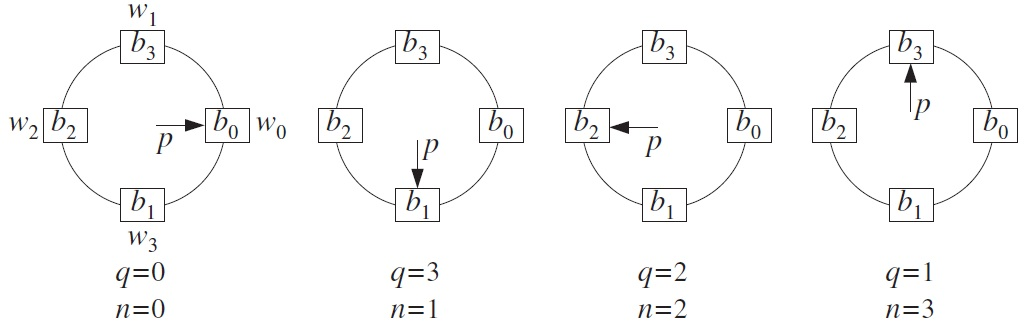
\includegraphics[width=\linewidth]{images/SignProcApp_Wavetable.jpg}
\end{center}

The wave can easily be delayed by $m$ time units by setting
\begin{equation*}
	y(n) = b(n-m)
\end{equation*}
This is achieved by initializing $p$ and $q$ with
\begin{equation*}
	p = w+m \quad q=m
\end{equation*}

This leads to the following sequences for different $m$'s

\begin{align*}
	m=0 \quad &[b_0,b_1,b_2,b_3,b_0,b_1,b_2,b_3,b_0,b_1,b_2,b_3,\ldots] \\
	m=1 \quad &[b_3,b_0,b_1,b_2,b_3,b_0,b_1,b_2,b_3,b_0,b_1,b_2,\ldots] \\
	m=2 \quad &[b_2,b_3,b_0,b_1,b_2,b_3,b_0,b_1,b_2,b_3,b_0,b_1,\ldots] \\
	m=3 \quad &[b_1,b_2,b_3,b_0,b_1,b_2,b_3,b_0,b_1,b_2,b_3,b_0,\ldots]
\end{align*}

The wavetable information can be manipulated in many possible ways to achieve
particular effects. A wavetable of length $D$ has a fundamental frequency $f$
of $f = \frac{f_s}{D}$. A shorter period $d \leq D$, meaning a higher frequency
$f = \frac{f_s}{d}$ can easily be achieved by skipping samples. \\

The constant $c = \frac{D}{d}$ describes, how often the sub-period $d$ fits into the original period $D$. To keep $f$ within the symmetric Nyquist interval, $c$ has to be inside the range

\begin{equation*}
	-\frac{D}{2} \leq c \leq \frac{D}{2}
\end{equation*}.

The update of the offset $q$ is
\begin{equation*}
	q_{n+1} = \left( q_n - c \right) \% D
\end{equation*}

Non-integer offsets can be truncated, rounded or, if higher quality is needed, interpolated.


\subsection{Noise Reduction and Signal Enhancement\buchSeite{382}}
Goal: extracting a signal from a noisy measurement. \\

\begin{tabularx}{\linewidth}{lX}
	Noisy measurement & $x(n) = s(n) + \nu(n)$ \\
	Desired signal & $s(n)$ \\
	Undesired noise & $\nu(n)$ \\
\end{tabularx} \\

\subsubsection{Noise Reduction Filters\buchSeite{382-386}}

The ideal noise reduction filter creates the output
\begin{equation*}
	y(n) = y_s(n) + y_{\nu}(n) \quad \text{with} \quad
		\begin{array}{l}
		y_s(n) = s(n) \\
		y_{\nu}(n) = 0
		\end{array}
\end{equation*}

The power spectral density of the output is calculated as
\begin{equation*}
	S_{yy}(\omega) = \left| H(\omega) \right|^2 S_{xx}(\omega)
\end{equation*}

with
\begin{equation*}
	\left| H(\omega) \right|^2 = H(\omega) \cdot H^*(\omega)
\end{equation*}

and with white noise as the input $S_{xx} = \sigma_x^2$
\begin{equation*}
	S_{yy}(\omega) = \left| H(\omega) \right|^2 \sigma_x^2
\end{equation*}

Not that the output noise is not white anymore and is therefore colored noise. \\

The \emph{noise reduction ratio} $\NRR$ measures the noise power at the output
compared to the noise power at the input. Note that a small NRR means
large noise reduction.
\begin{equation*}
	\NRR = \frac{\sigma_y^2}{\sigma_x^2}
		 = \int\limits_{-\pi}^{\pi} \left| H(\omega) \right|^2 \frac{d\omega}{2\pi}
		 = \sum\limits_{n} h(n)^2
\end{equation*}

The \emph{signal to noise ratio} $\SNR$ can be calculated at the input and
at the output, hence the relative improvement of the SNR is
\begin{equation*}
	\frac{\SNR_{\text{out}}}{\SNR_{\text{in}}} = \frac{1}{\NRR} \cdot \frac{E\left[y_s(n)^2\right]}{E\left[s(n)^2\right]}
\end{equation*}

or if the desired signal $s(n)$ is not changed by the filter
\begin{equation*}
	\frac{\SNR_{\text{out}}}{\SNR_{\text{in}}} = \frac{1}{\NRR}
\end{equation*}

The best possible $\NRR$ is achieved by using ideal filters:

\begin{tabularx}{\linewidth}{lX}
	Ideal lowpass filter & $\NRR = \frac{\omega_c}{\pi}$ \\
	Ideal bandpass filter & $\NRR = \frac{\omega_b - \omega_a}{\pi}$ \\
\end{tabularx} \\

Most real noise reduction filters are linear phase filters, where each frequency is delayed by the same number of samples and implies constant phase delay:
\begin{align*}
  y_s(n) = s(n-D)
\end{align*}

\paragraph{First-order IIR Smoother\buchSeite{386}}
To remove zero-mean white Gaussian noise of variance $\sigma_v^2$, an
IIR lowpass filter is used:
\begin{equation*}
	H(\z) = \frac{b}{1-a\z^{-1}}
\end{equation*}

With $0 < a < 1$ and $H(1)=1$, $b$ can be fixed to $b=1-a$. In that
case the $\NRR$ is
\begin{equation*}
	\NRR = \frac{b^2}{1-a^2} = \frac{1-a}{1+a}
\end{equation*}

The transient time constant will be
\begin{equation*}
	n_{\text{eff}} = \frac{\ln \epsilon}{\ln a} \to \infty \quad \text{as} \quad a \to 1
\end{equation*}
The one-percent time constant is of course
 $n_{\text{eff}}=\frac{\ln(0.01)}{\ln(a)}$ \\

The 3-DB cutoff frequency $\omega_c$ is calculated at
$\left| H(\omega_c) \right|^2 = \frac{1}{2}$, leading to
\begin{equation*}
	\omega_c = 1 - \frac{(1-a)^2}{2 a} \stackrel{\text{for } a \lesssim 1}{\backsimeq} 1-a
\end{equation*}

\paragraph{Highpass signal extraction filter\buchSeite{389}}
The $\NRR$, $n_{\text{eff}}$ and $\omega_c$ for a highpass IIR filter with
\begin{equation*}
	H(\z) = \frac{b}{1+a\z^{-1}}
\end{equation*}
can be calculated similarly, leading to the same results:
\begin{equation*}
	\NRR = \frac{1-a}{1+a} \qquad n_{\text{eff}} = \frac{\ln \epsilon}{\ln a} \qquad \omega_c \lesssim 1-a
\end{equation*}

\paragraph{First-order IIR smoother with prescribed cutoff frequency\buchSeite{390}}
By adding a zero at $\z=-1$, the $\NRR$ can be slightly improved.
The filter will be
\begin{equation*}
	H(\z) = \frac{b \left( 1 + \z^{-1} \right)}{1 - a \z^{-1}}
\end{equation*}
with $b = \frac{1-a}{2}$ for unity gain at DC. The NRR of this filter will be
\begin{equation*}
	\NRR = \frac{1-a}{2}
\end{equation*}
The following equations are used to determine $\omega_c$ or $a$.
\begin{equation*}
	\cos \omega_c = \frac{2 a}{1+a^2} \Leftrightarrow a = \frac{1-\tan(\omega_c/2)}{1+\tan(\omega_c/2)}
\end{equation*}

\paragraph{FIR averaging filters\buchSeite{391}}
For a FIR filter, the $\NRR$ will always be
\begin{equation*}
	\NRR = \sum\limits_n h_n^2
\end{equation*}
A filter minimizing the $\NRR$ is obtained by setting $h_n = \frac{1}{N}$, which is a simple averaging filter. The $\NRR$ will be
\begin{equation*}
	\NRR = \frac{1}{N}
\end{equation*}
The length $N$ of a FIR filter should be chosen like the time constant
$n_{\text{eff}}$ for an IIR filter:
$N = n_{\text{eff}} = \frac{\ln \epsilon}{\ln a}$ \\

The cutoff frequency of an FIR averaging filter is
\begin{equation*}
	\omega_c = \frac{\pi}{N}
\end{equation*}

\paragraph{Highpass FIR signal extraction\buchSeite{396}}
The lowpass filter is changed to a highpass filter by substituting $\z \to -\z$,
changing the impulse response to $h_n \to (-1)^n h_n$, leading to
a highpass FIR filter with the impulse response
\begin{equation*}
	h_n = (-1)^n \frac{1}{N}
\end{equation*}
The noise reduction ratio stays the same.

\paragraph{Bandpass signal extraction\buchSeite{397}}
A FIR bandpass filter is achieved by a resonator filter with poles at $z = R e^{\pm j \omega_0}$.
\begin{align*}
	H(\z) &= \frac{G}{1 + a_1 \z^{-1} + a_2 \z^{-2}} \\
	h_n &= \frac{G}{\sin \omega_0} R^n \sin\left(\omega_0 n + \omega_0\right) u(n)
\end{align*}
where $a_1 = -2R \cos\omega_0$ and $a_2 = R^2$. \\

The $\NRR$ of this filter will be
\begin{equation*}
	\NRR= \frac{(1-R)(1+R^2)(1-2R\cos(2\omega_0)+R^2)}{(1+R)(1-2R^2\cos(2\omega_0)+R^4)}
\end{equation*}

The recovered sinusoid will be shifted by the phase delay $d$ of
\begin{equation*}
	d(\omega_0) = - \frac{\arg H(\omega_0)}{\omega_0}
\end{equation*}


\subsubsection{Notch and Comb Filters\buchSeite{398-406}}

Two special cases of the signal enhancement/noise reduction problem arise when:
\begin{enumerate}
	\item The noise signal $\nu(n)$ is periodic. The ideal filter will then
	be a notch filter.
	\item The desired signal $s(n)$ is periodic. The ideal filter will then
	be a comb filter.
\end{enumerate}

Usually all the harmonics of the fundamental frequency $f_1$ must be canceled.
The sampling rate $f_s$ is then chosen to be a multiple $f_1$:
\begin{equation*}
	f_s = D f_1
\end{equation*}
The noise harmonics then occur at the $D^{\text{th}}$ roots-of-unit frequencies:
\begin{equation*}
	f_k = k \frac{f_s}{D}
\end{equation*}

\paragraph{Notch filters}The notch filter is then given by
\begin{equation*}
	H_{\text{notch}}(\z) = b \frac{1-\z^{-D}}{1-a\z^{-D}}
\end{equation*}
with $b = \frac{1+a}{2}$ and $a = \rho^D$. Again $a$ must be in the interval
$0 \leq a < 1$. \\

For a given $\Delta\omega$ of the notch dips, $a$ and $b$  are obtained by
\begin{equation*}
	\beta = \tan\left(\frac{D\Delta\omega}{4}\right) \qquad a = \frac{1-\beta}{1+\beta} \qquad b = \frac{1}{1+\beta}
\end{equation*}

\paragraph{Comb filters}
As a multi-notch filter can be obtained from a single notch filter using the
substitution $\z \to \z^D$, which creates $D$ replicas in the Nyquist band,
any narrow lowpass filter can be transformed into a comb filter.
\begin{equation*}
	H(\z) = b \frac{1+\z^{-1}}{1-a\z^{-1}} \quad \to \quad
	H_{\text{comb}}(\z) = b \frac{1+\z^{-D}}{1-a\z^{-D}}
\end{equation*}

Given a 3-dB width for the peaks, the parameters can be calculated by
\begin{equation*}
	\beta = \tan\left(\frac{D\Delta\omega}{4}\right) \qquad
	a = \frac{1-\beta}{1+\beta} \qquad b = \frac{\beta}{1+\beta}
\end{equation*}

Note that the presented notch and comb filters are complementary, i.e.
\begin{equation*}
	\left|H_{\text{comb}}(\omega)\right|^2 + \left|H_{\text{notch}}(\omega)\right|^2 = 1
\end{equation*}

The $\NRR$s are the same as the $\NRR$s for the simple smoothers, as the
transform $\z \to \z^{D}$ simply inserts $D-1$ zeros in the original
impulse response. Hence the sum does not change and the $\NRR$s don't change.


\subsubsection{Signal Averaging\buchSeite{421-427}}
Signal averaging is equivalent to comb filtering, but with an FIR filter
instead of an IIR one. It is derived by applying the transform $\z \to \z^{-1}$
to the FIR averaging filter of length $N$:

\begin{align*}
	H(\z)&=\frac{1}{N}\left( 1+ \z^{-D}+\z^{-2D}+\ldots + \z^{-(N-1)D} \right) \\
	&= \frac{1}{N}\frac{1-\z^{-ND}}{1-\z^{-D}}
\end{align*}

Again, the $\NRR$ stays the same: $\NRR = \frac{1}{N}$. \\

In the time domain, the filter is given by the following I/O difference equation:

\begin{equation*}
	y(n) = \frac{1}{N} \left[ x(n)+x(n-D)+\ldots+x(n-(N-1)D) \right]
\end{equation*}

As the IIR comb filter is more efficient, it is mostly used for real time
processing. The FIR averaging filter is used when measuring a finite number
$N$ of periods of the same noisy signal. \\

For $N$ periods of $D$ samples, the total length will be $ND$. The $i$th period
of the signal will then be
\begin{equation*}
	x_i(n) = x(iD+n)
\end{equation*}
where $i=0,1,\ldots,N-1$ for a total of $N$ periods. \\

The output will then be
\begin{equation*}
	\hat{y}(n)=\frac{1}{N}\sum_{i=0}^{N-1}x_i(n)
\end{equation*}

and the noise will, of course, be reduced by a factor of the $\NRR$, i.e.
\begin{equation*}
	\sigma_{\hat{v}}^2 = \frac{1}{N} \sigma_v^2
\end{equation*}


\subsubsection{Savitzky-Golay Smoothing Filters\buchSeite{427-451}}

The Savitzky-Golay smoothing filters (also: polynomial smoothing or
least-squares smoothing filters) are an elegant generalization of the
simple FIR averaging filter. \\

It optimally fits a set of data points to a polynomial of a specified
degree in least-squares sense.

\begin{center}
	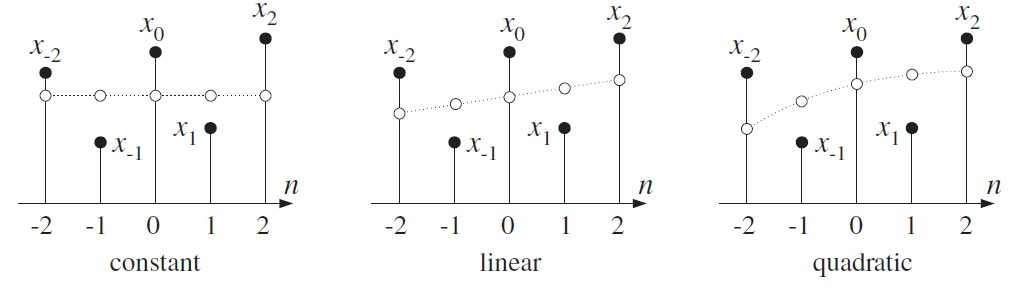
\includegraphics[width=\linewidth]{images/SignProcApp_SavitzkyGolay.jpg}
\end{center}

The smoothed value $\hat{x}_m$ at each point is given by
\begin{equation*}
	\hat{x}_m = c_0 \qquad \hat{x}_m = c_0 + c_1 m \qquad \hat{x}_m = c_0 + c_1 m + c_2 m^2
\end{equation*}
with the free variable $m = -2,-1,0,1,2$. \\

The coefficients $c_i$ now have to be
optimally found in a least-squares sense, using linear algebra. \\

We  therefore introduce \emph{basis vectors}
$\mathbf{s}_0, \mathbf{s}_1, \mathbf{s}_2$, whose components are (quadratic approx.):
\begin{equation*}
	\mathbf{s}_0(m) = 1 \qquad \mathbf{s}_1(m) = m \qquad \mathbf{s}_2(m) = m^2 \\
\end{equation*}
Therefore
\begin{equation*}
	\hat{\mathbf{x}} = \left[\mathbf{s}_0,\mathbf{s}_1,\mathbf{s}_2\right]
	\begin{bmatrix}c_0\\c_1\\c_2\end{bmatrix} = S\mathbf{c}
\end{equation*}
with the optimal coefficients
\begin{equation*}
	\mathbf{c} = G^T \mathbf{x} \qquad \text{with} \qquad G = S \left(S^T S \right)^{-1}
\end{equation*}
Inserting the optimal coefficients, we find
\begin{equation*}
	\hat{\mathbf{x}} = S G^T \mathbf{x} = B \mathbf{x} \quad \text{with} \quad B = S G^T = S \left(S^T S\right)^{-1} S^T
\end{equation*}

And therefore the output smoothed value
\begin{equation*}
	y_0 = \hat{x}_0 = c_0 = \mathbf{b}_0^T \mathbf{x} = \mathbf{g}_0^T \mathbf{x}
\end{equation*}

This can be realized as a regular FIR filter, which is in case of the 2nd order
polynomial
\begin{equation*}
	y_0 = \frac{1}{35} \left( -3 x_{n-2} + 12 x_{n-1} + 17 x_n + 12 x_{n+1} - 3 x_{n+2}\right)
\end{equation*}

The $\NRR$ of Savitzky-Golay filters is the middle coefficient:
\begin{equation*}
	\NRR = \mathbf{b}_0^T \mathbf{b}_0 = b_0(0) = \frac{17}{35} = 0.49
\end{equation*}

\paragraph{Savitzky-Golay for derivatives}
Focus on the middle value at $m=0$:
\begin{equation*}
	\hat{x}_m = c_0 + c_1 m + c_2 m^2
\end{equation*}
Clearly the derivatives are
\begin{align*}
	\dot{\hat{x}}_0 &=  \left.\frac{d\hat{x}_m}{dm}\right|_0 = c_1 = \mathbf{g}_1^T\mathbf{x} \\
	\ddot{\hat{x}}_0 &= \left.\frac{d^2\hat{x}_m}{dm^2}\right|_0 = 2 c_2 = 2 \mathbf{g}_2^T\mathbf{x}
\end{align*}
and can be written as FIR filters
\begin{align*}
	\dot{y}_n &= \frac{1}{35} \left( -7 x_{n-2} - 3.5 x_{n-1} + 3.5 x_{n+1} + 7 x_{n+2}\right) \\
	\ddot{y}_n &= \frac{2}{35} \left( 5 x_{n-2} - 2.5 x_{n-1} - 5 x_n - 2.5 x_{n+1} + 5 x_{n+2}\right)
\end{align*}

\paragraph{Savitzky-Golay for integrals}
The same concepts of course also apply to  the integral $i$:
\begin{align*}
	i_n &= \int\limits_{-1/2}^{1/2} \hat{x}_m dm = \int\limits_{-1/2}^{1/2} (c_0 + c_1 m + c_2 m^2) dm \\
	&= \left[1 \: 0 \: 1/12 \right] \cdot \mathbf{c} = \left[1 \: 0 \: 1/12 \right] \left(S^T S \right)^{-1} S^T \mathbf{x}
\end{align*}
which leads to
\begin{align*}
	\dot{y} = & \left(-0.0738 x_{n-2} + 0.3369 x_{n-1} + \right. \\
	& \left. 0.4738 x_n + 0.3369 x_{n+1} - 0.0738 x_{n+2}  \right) \\
\end{align*}

\paragraph{Generalization}
So far, the length was $N=5$ and the degree $d=2$. Of course this can easily be
generalized to any odd $N \geq d+1$.
\begin{align*}
  N &= 2M + 1 \\
  \mathbf{x} &= [x_{-M},\ldots,x_{-1},x_0,x_1,\ldots,x_M]^T \\
  \hat{x}_m &= c_0 + c_1m + \ldots + c_dm^d, \quad -M \leq m \leq M
\end{align*}
